\documentclass[14pt]{extreport}

\usepackage{geometry}
\usepackage{graphicx}
\usepackage{dcolumn}
\usepackage{bm}
\usepackage{pythonhighlight}
\usepackage{tikz}
\usepackage{tikz-cd}
\usepackage{pgfplots}
\usepackage{multirow}
\usepackage[hidelinks]{hyperref}
\usepackage{times}
\usepackage{setspace}
\usepackage{amsmath}
\usepackage{amsfonts}
\usepackage{amssymb}
\usepackage{amsthm}
\usepackage{bbold}
\usepackage{color}
\usepackage{soul}

\doublespacing
\geometry{margin=0.75in,top=1in, bottom=0.9in}
\pgfplotsset{compat=1.14, scale = 0.25}

\renewcommand{\thesection}{\arabic{section}}

\setlength{\topskip}{-1cm}

\title{An Investigation of Deep Learning Models for Image Enhancement in MRI}
\author{Evan M. R. Petrimoulx}
\date{\today}

\renewenvironment{abstract}{
    \begin{center}
        \bfseries Abstract
    \end{center}
    \vspace{-1em} % Adjust this to reduce space
    \itshape
}{}

\begin{document}
    \maketitle
    \setcounter{page}{2}
    \vspace{-2cm}
    \begin{abstract}
        \indent Since its invention, MRI has been an essential tool in imaging samples and diagnosing patients. While the results from an MRI scan are crucial in providing doctors and researchers clear images of \hl{their} sample, it can take hours to gather the necessary k-space data to produce useful images. A rising technique to help combat the large scan times and image processing times is to implement deep learning models. These neural networks are capable of learning from the data in the frequency domain across multiple training scans and predict the images produced from new samples given a restricted k-space domain. Reducing k-space sampling shortens scan times but often degrades image quality, introducing aliasing and contrast loss. Teaching a neural network the trends and patterns present in the frequency domain for a sample can help generate images with close to the same image quality as that produced with a full frequency spectrum scan. Correctly training these models allows for the reconstruction of high-quality images from undersampled scans. Convolutional Neural Networks (CNNs), a common feedforward model used in image processing, are particularly effective for MRI enhancement and reconstruction, and are the standard model used in the field. This report investigates the different techniques and implementation strategies of these models in MRI, and discusses the advantages as well as the limitations of these models. Furthermore, this report provides examples of neural networks which showcase the capability of image reconstruction, as well as the issues present with them such as overfitting, which can cause hallucinations that are present in the final generated image and must be avoided.
    \end{abstract}

    \section*{Introduction}
        \indent Magnetic Resonance Imaging (MRI) is an imaging technique that utilizes the resonant frequency of atoms, typically hydrogen, as well as strong external gradient magnetic fields to produce image slices of a subject. The process of recovering an image given a measurement of frequency represented as a signal is done by performing the inverse Fourier Transform to the measured signal.

        \begin{align}
            \rho(x) = \mathcal{F}^{-1}\{ S(k) \} = \int_{-\infty}^{\infty} S(k) e^{i 2\pi k x} \;dk\;. \label{fft}
        \end{align}

        The problem lies within the collection of signal data in the frequency domain. If the entirety of the frequency domain is not sampled, then key data pertaining to the image reconstruction is lost. This typically leads to loss of contrast in the image, as well as decreased image sharpness, and can cause aliasing. 
        
        \begin{figure}[h]
            \begin{center}
                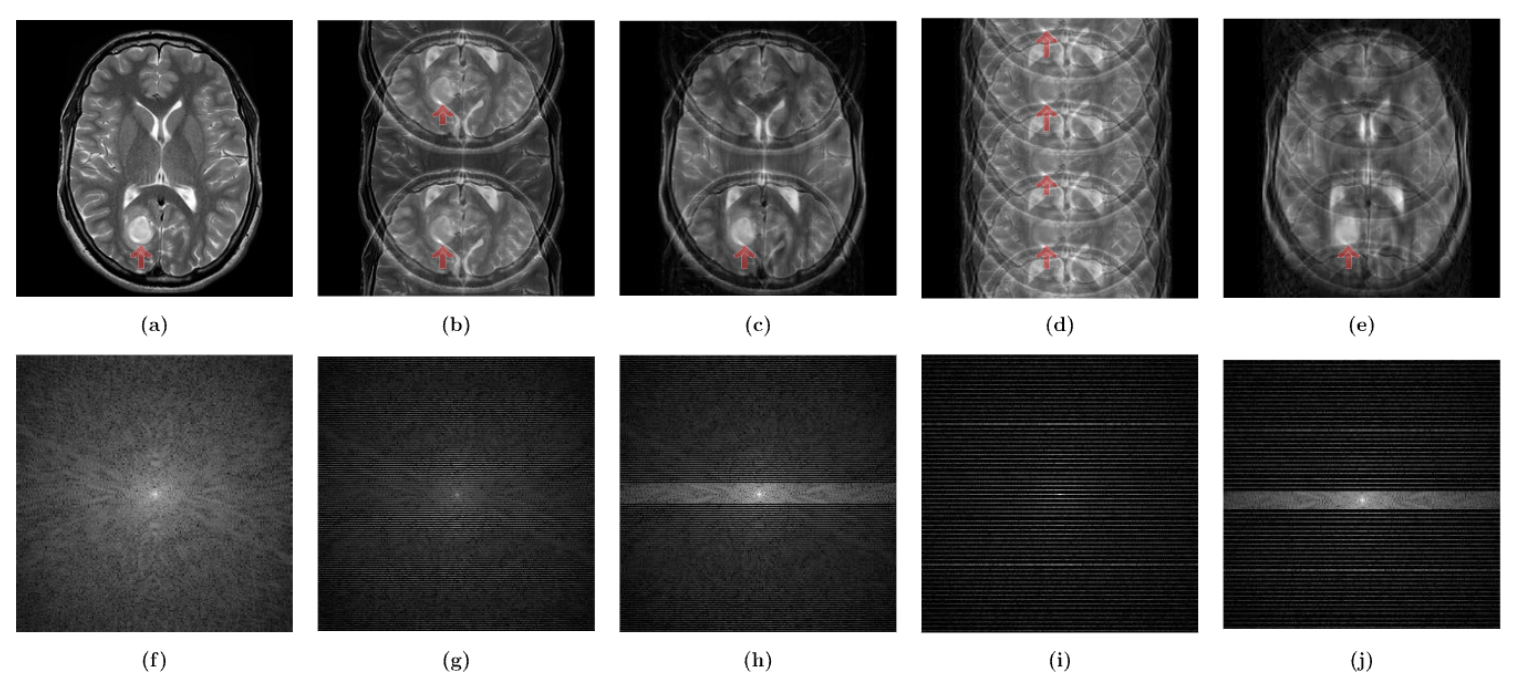
\includegraphics[width = \linewidth]{Brain Images.png}
                \caption{Image of a human brain from \cite{Hyun_Kim_Lee_Lee_Seo_2018}. As the frequency domain data collection is reduced, the image quality becomes worse and aliasing occurs.}
            \end{center}
        \end{figure}

        MRI relies on the relaxation time of isochromats tending back to equilibrium after being aligned with the external field. Because of this, rapid data acquisition is constrained by $T_1$, $T_2$, and $T_2^*$ signal decay times. As a result, obtaining a full k-space dataset requires significant time, causing a negative relationship between image clarity and speed. Finding techniques that allow for less frequency domain to be required \hl{would therefore} decrease scanning times, and maintain image quality. This would allow for hospitals to see more patients more frequently at a cheaper cost of diagnosis. One of these methods is the implementation of \hl{neural networks}. Neural networks are a category of machine learning that is modelled after the human brain \cite{Pytorch_Book}. They are capable of complex pattern recognition and extrapolation which can be used to successfully construct a high quality image given a reduced amount of k-space data \cite{Hammernik_Klatzer_Kobler_Recht_Sodickson_Pock_Knoll_2018}. Successfully training a neural network to identify patterns in k-space data allows researchers to spend less time performing data aquisition in the frequency domain, while still retaining quality in the image domain.
    
    \section*{Theory}
        In order to understand how neural networks work, it is helpful to start with a simpler model. Machine learning as a whole can roughly be separated into two categories, \hl{regression} and \hl{classification}. Classification problems deal with the identification of discrete data. This is common for solving problems such as image identification. Classification algorithms can identify things like handwriting, or parts of the human body given an image. Classification is used to model discrete data. Regression is the opposite. Regression models in machine learning deal with identification of trends or continuous data. \hl{Regression models, sometimes referred to as regressors}, are capable of predicting trends such as in price changes in the stock market, or rate of spread of disease. Both models require large amounts of data for training. In order for these models to learn, they must be given data involving many features (variables) and a known output. When the output of the function being analized is known, the development of the model is called supervised learning. These models then analyze the trends \hl{via the relationships} between the features presented in the dataset, and find a complex equation that it deems worthy of accurately representing the data it was presented. For the problem of image enhancement in MRI, regressors are the correct tool for the problem since a continuous amount of data from the frequency domain is needed to reconstruct an image. 

        In the event that the data presented to the model is more complex than a linear relationship, the model will have a difficult time predicting an output\cite{Raschka_2022}. To solve this issue and allow for the analysis of higher order correlations in data, the features can be processed through intermediate relationships called layers. For a single layer, the problem is linear and any simple regressor can predict an output. When there is more than one layer present in the model, the machine learning algorithm is referred to as a deep learning model. Neural Networks are a form of deep learning model where each feature in the data set is connected to other features in a web across multiple layers. The mathematical relationship between a single neuron \hl{(a node within the layer of the neural network)} in the network is given by the following equation \cite{Gazit_2024}\hl{:}
        
        \begin{align}
           y = f\left(\sum_{i = 1}^n w_i x_i + b \right) \;.
        \end{align}

        Where $f$ is the activation function which is dependant on \hl{the weighting of each linear feature for each neuron $w_i$}, the feature or variable itself $x_i$, and the bias term $b$, which tells the algorithm how important a value is to the pattern it is finding \hl{and is common to all weighting parameters}. The summation sums over all of the features that are interconnected in the layer. Training a neural network requires adjusting the weights and biases of the nodes (neurons) to minimize a loss function via an optimization algorithm such as gradient descent. 
        
        A loss function is a function that takes two inputs and computes how similar they are to one another. The more similar the two values are, the more the model is able to predict given the trend it has discovered. The average loss over the entire dataset can tell us how correct our model is. It is given by the following formula\hl{:}
        
        \begin{align}
            \langle L_{\text{total}}(y, \hat{y}) \rangle = \frac{1}{N} \sum_{i = 1}^N L(y, \hat{y})\;.
        \end{align}

        Where there are $N$ variables or features in the dataset and $L(y, \hat{y})$ is the loss function\hl{,} $y$ is our prediction value\hl{,} and $\hat{y}$ is the known correct value \cite{Hoyle_2024}. The loss function and its minimization are what makes the neural network capable of learning nonlinear trends. This is one of the advantages of deep learning models compared to linear regression models such a ridge regression. There are many different possible loss functions that are dependant on the statistics of the machine learning model being used, but a common example is the least squares loss function. This has the typical definition for least squares fitting \cite{Hoyle_2024}
        
        \begin{align}
            f_{\text{lsqf}} = \left(y - \hat{y} \right)^2\;.
        \end{align}
        %
        The more layers that are present, the more complex the neural network model becomes. By learning to reconstruct undersampled k-space data, deep learning effectively approximates the missing frequency components. This allows it to find deeper connections between the signals in k-space, but has the risk of introducing a flaw if the model is too complex; overfitting. 

        \begin{figure}[h]
            \begin{center}
                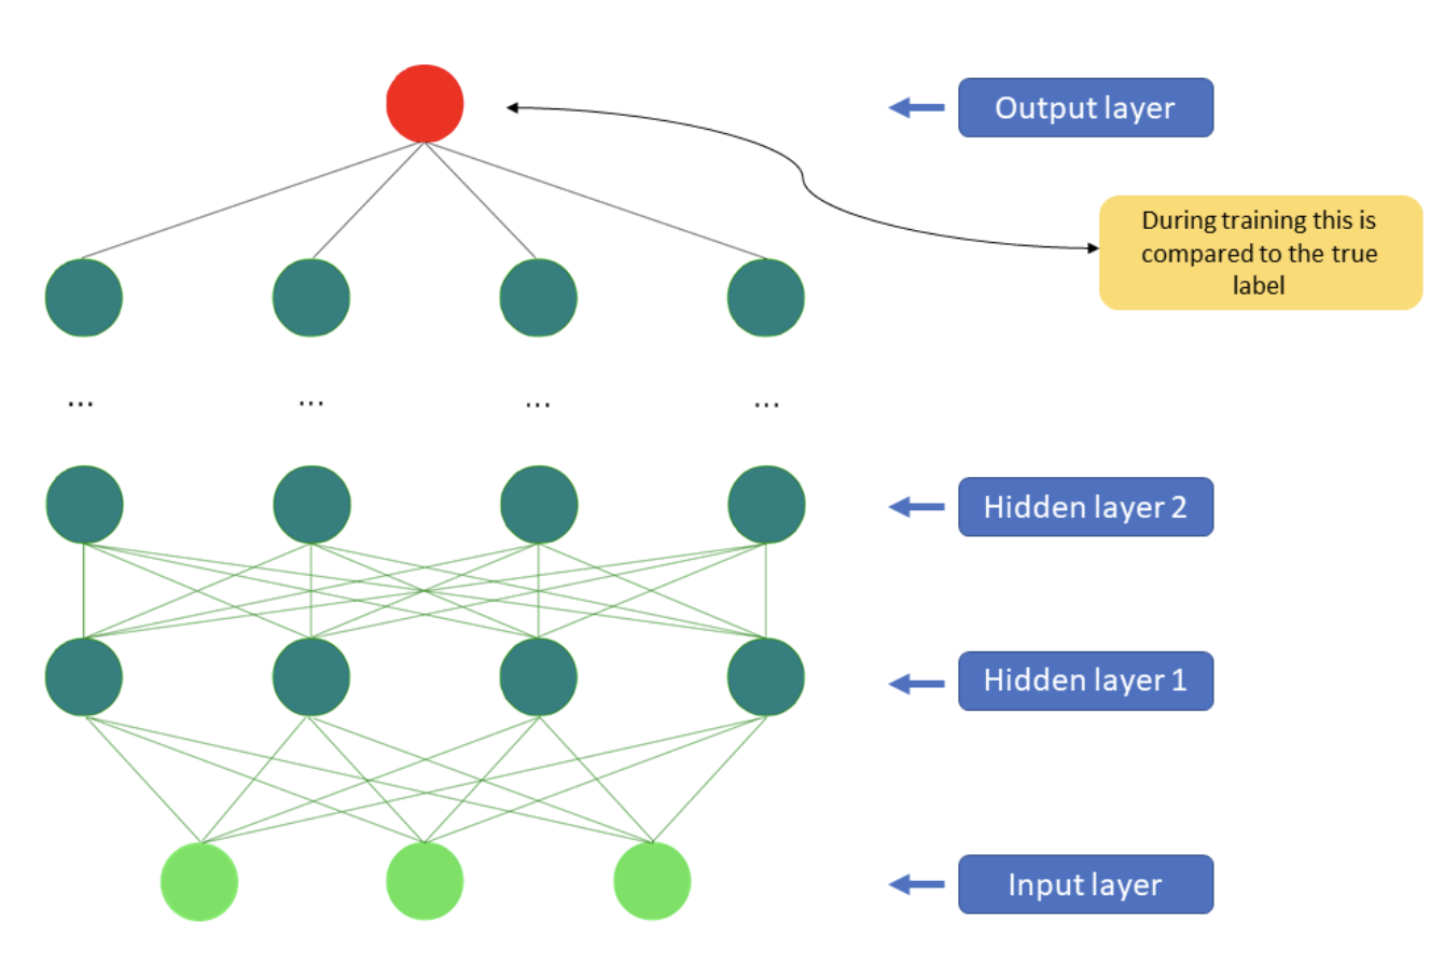
\includegraphics[width = 0.6\linewidth]{Neural Network.png}
                \caption{Image from \cite{Lundervold_Lundervold_2019} depicting the graphical representation of a deep learning neural network}
            \end{center}
        \end{figure}

        In the event that a neural network contains too many layers, its ability to analyze data becomes increasingly complex. When this happens, the model starts to memorize specific patterns in the training data, rather than learning generalizable trends. In other words, the model learns too much from the dataset such that it starts to make predictions that are biased towards the data it is trained on. This is known as overfitting, and when applied to an image processing algorithm, can be referred to as hallucinations. When the model learns too deeply about its training data, it may start to predict patterns that are specific to only the training data, and not anything in nature or any real pattern. The model then tries to impose these features onto other problems when they shouldn't be there. A model trained on mice brains when presented with the \hl{brain of a rat} may try to enhance the image of the rat brain by imposing features of the mice brains it studied onto the image\hl{;} this is called a hallucination. Training a model effectively involves not only training it with a given dataset, but ensuring that the model does not become too complex and bias your output data. This is crucial in the implementation for MRI scans, since a biased model may hide important features of the image such as tumours that doctors or researchers are looking for. However, if the model is correctly trained and does not overfit, \hl{it can be given} some frequency domain data that is undersampled \hl{which} does not contain the entire spectrum, and the model will regenerate a correct image that can be analyzed, \hl{as shown by} \cite{Hyun_Kim_Lee_Lee_Seo_2018}. This can save time and memory usage on the computer when processing MRI scans\hl{,} allowing for quicker scan times and faster image processing for less computational cost \cite{Hyun_Kim_Lee_Lee_Seo_2018}. 

        \begin{figure}[h]
            \begin{center}
                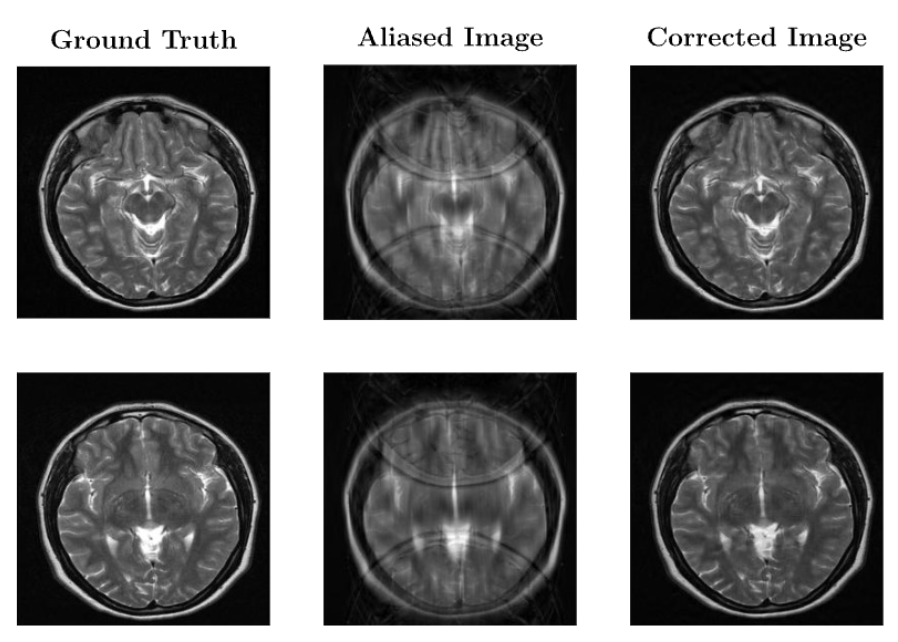
\includegraphics[width = 0.6\linewidth]{Brain Images Corrected.png}
                \caption{Example of MRI image reconstruction using a deep learning model, showing improved contrast and reduced aliasing \cite{Hyun_Kim_Lee_Lee_Seo_2018}.}
            \end{center}
        \end{figure}

        Another way to help prevent overfitting is by using Convolutional Neural Networks (CNNs). CNNs are a specific archetype of neural networks with a slightly different layering scheme. Since the \hl{more layers} that are present in the network, the more complex the algorithm is, we can reduce the number of compared functions for each node in the layer to provide less complex data to the model. This keeps the nonlinear capabilities of the model by keeping many layers, but removes the likelihood of overfitting by supplying less data at each iteration. A convolutional neural network does this by forming two different types of layers; a convolution layer and a pooling layer. 

        The convolutional layer only compares a few nodes with \hl{each other}, typically a small patch of $3\times3$ nodes \cite{Liu_Pan_Li_Chen_Tang_Lu_Wang_2018}. This allows for each feature being compared in the smaller layer to hold more impact, and its correlation between the features to be more pronounced. This provides insight on the correlation between a few features, instead of trying to compare all features at once.

        The pooling layer comes after the convolutional layer has been computed, and simplifies the number of parameters in the function. This is typically done by reducing the size of the feature matrix being passed in to the layer. A reduced system of feature equations to be solved means less computation time and less complexity, further reducing the chances of overtraining the model and causing hallucinations.

    \section*{Methods}
        \hl{In order to begin training a CNN, a model must first be chosen}. For this report, tensorflow \hl{was} utilized as the main machine learning library in conjunction with scikit-learn. Tensorflow is a machine learning library built by Google, and contains many useful features that allow for simple setup of a CNN, such as MaxPooling2D, which allows for the pooling process of 2-dimensional data. This is particularly useful for when we pass 2D k-space data to the neural network. \hl{All models were trained on an Apple Macbook air M2 with 16Gb of unified memory.}

        First, the dataset \hl{was} downloaded. This project uses the IXI dataset \cite{IXI_Dataset}, which contains MRI image data from various hospitals in England. The dataset provides \hl{$T_1$ and $T_2$} weighted images, but the focus of this project will mainly be on $T_1$ weighted images. The datasets are quite large (around 11Gb each), so to limit the size and training time of the model, the data for $T_1$ weighted images \hl{was} saved and stored in a compressed CSV called a parquet. Next, the data is converted to a dataframe in pandas for easy data manipulation. From here, the desired slices from the 581 different images present are stored in a separate data file for processing. \hl{Five} slices at a similar depth are gathered for each patient in order to increase the data available to the model, but many slices are discarded since the focus of this project is brain scans, not the entire skull. Discarding slices far away from the point of interest helps the model focus on learning brain images, and not become confused about a slice containing frequency data for a jaw\hl{, for example}. 

        Now that the data has been gathered correctly, a second dataset is constructed identical to the first. Since all of the data processed so far is from the IXI dataset, there is no undersampled k-space data. Here, all photos are randomly sampled and have regions of high-frequency k-space removed from them. This random approach removes any bias from the user when creating undersampled images. The low frequency ranges are prioritized here since they contain the most important pieces of information. This artificial undersampled data serves as our testing data for the model. 

        Once the frequency data for the desired 2D slices is gathered, the real and imaginary parts of the k-space data are split up. This is necessary since most CNN models do not accept complex data. To work around this, the imaginary part of the data is stored as if it was a second real value, and then is recombined at the end of running the CNN with the real part of the data to successfully reconstruct the image. From here, many combinations of layers, iterations, batches, and epochs are tested as well as the intensity of the undersampling. \hl{A batch is a dataset that has been divided into smaller parts to be given to the network, and an epoch is the complete analysis of all of the batches at once.} The images are then gathered and model accuracy is evaluated \hl{using the mean squared error, as well as expressing the number of correct predictions versus incorrect predictions as a percentage}. This process is repeated at different intensities for the model to test for underfitting, overfitting, and generalization. It is important to note here that the dataset only contains 581 images. Most neural networks require thousands of images to learn effectively, and the model may have reduced performance due to the lack of data. This is countered by having high learning rates \hl{(the amount of learned information passed from one layer to the next, expressed as a percentage of the total information gathered)} from pixel to pixel in the neural network, with many iterations through the data.

    \section*{Discussion and Results}
        After training many models on the artificially undersampled IXI dataset, it was found that the models were able to successfully learn from the frequency space data and recreate the MRI image scans. Two examples are shown displaying the predictive power of the CNN and its ability to reconstruct missing k-space data in figures \ref{img:kspace-1} and \ref{img:kspace-2}. \hl{Given a medium intensity undersampled k-space, the frequency data was successfully reconstructed, leading to a reconstructed image space which resembles the original image of the patient without undersampled k-space data. The additional blurring to the image is due to the model's dataset being quite small, likely causing underfitting.}

        \begin{figure}[h]
            \centering
            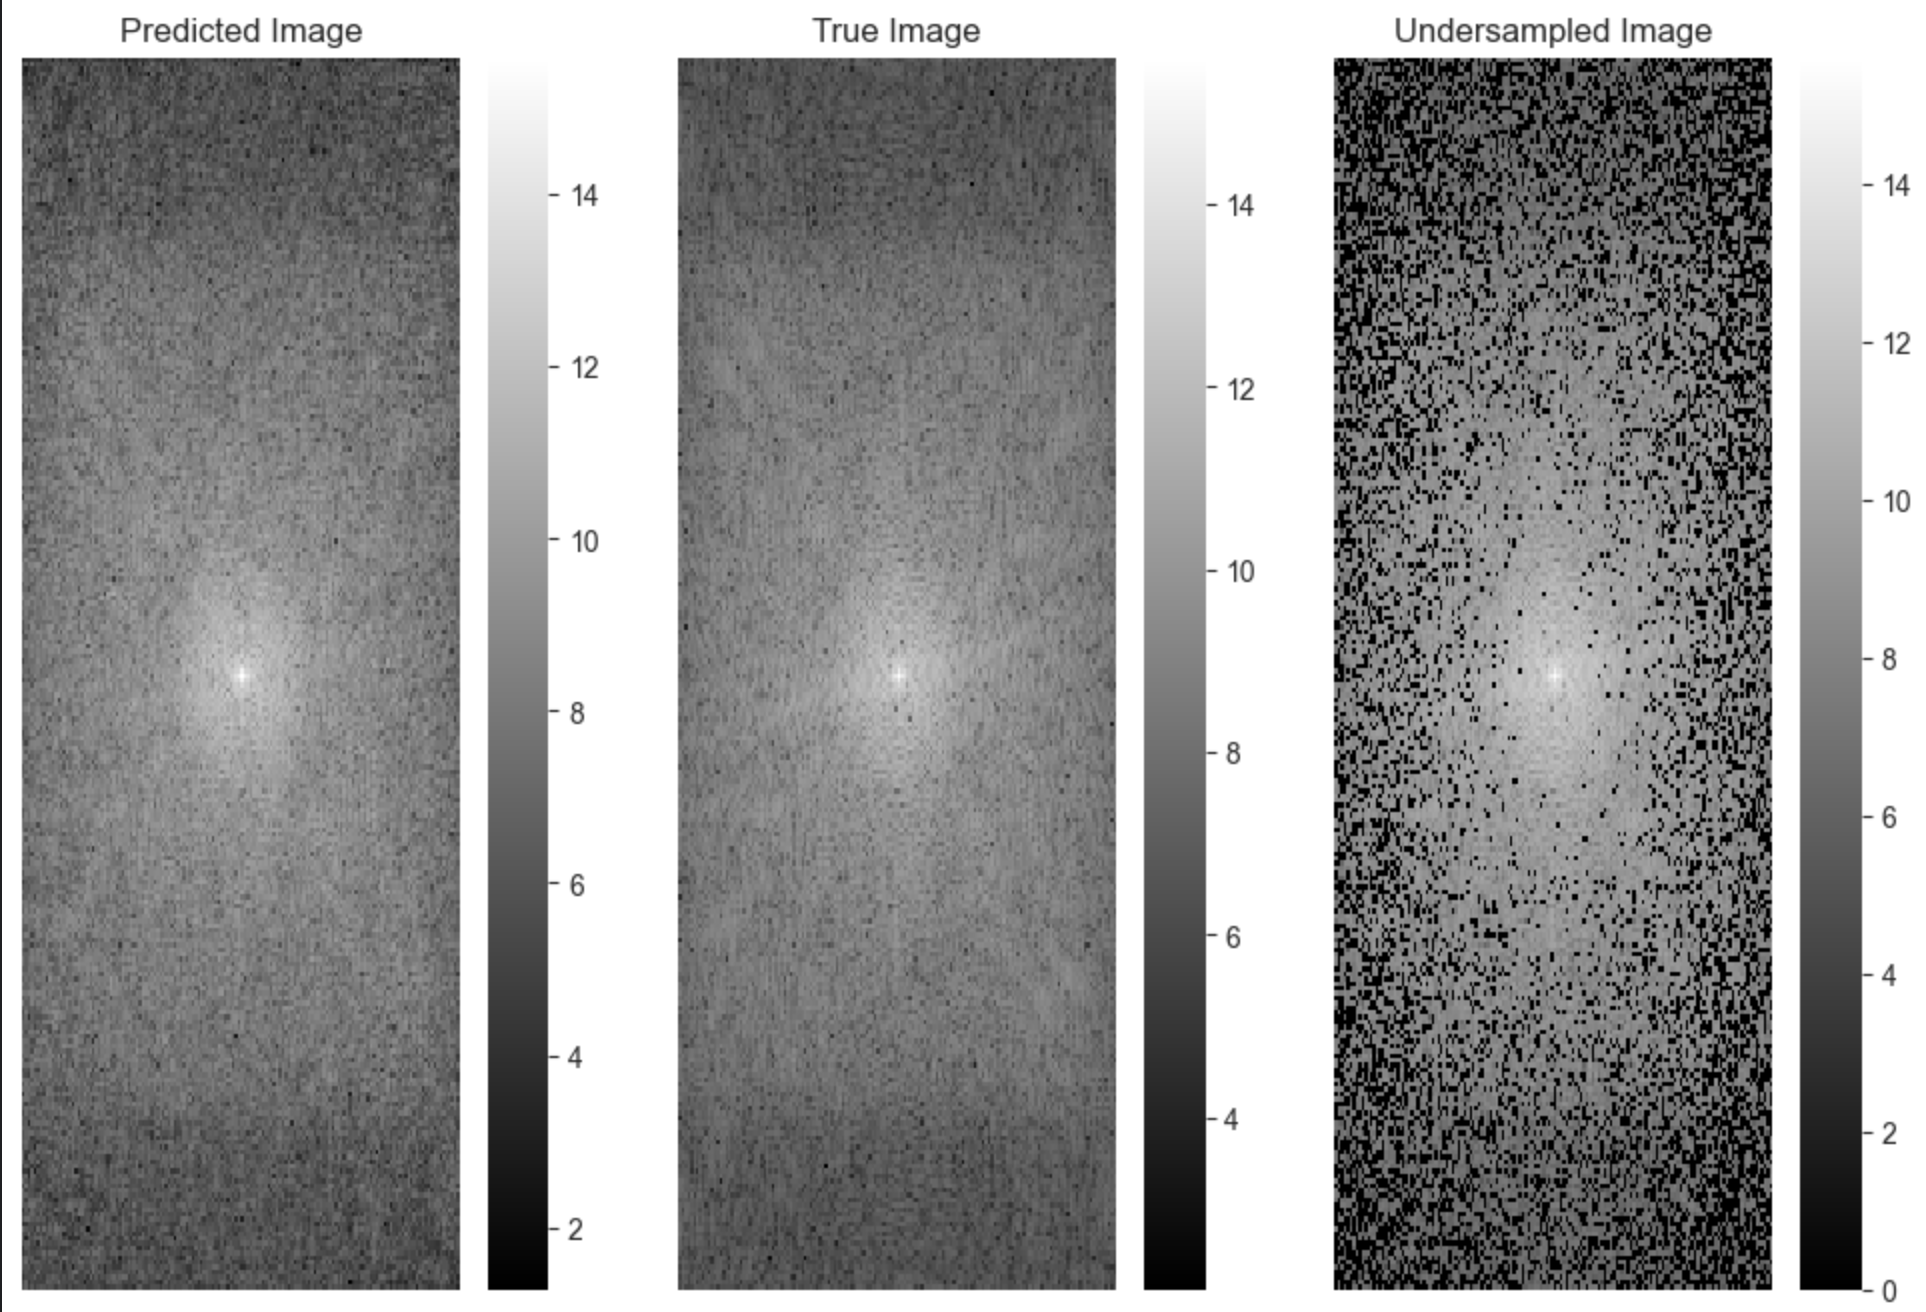
\includegraphics[width=0.75\linewidth]{CNN_1_kspace.png}
            \caption{k-space reconstruction using a CNN for medium intensity undersampled k-space.}
            \label{img:kspace-1}
        \end{figure}

        \begin{figure}[h]
            \centering
            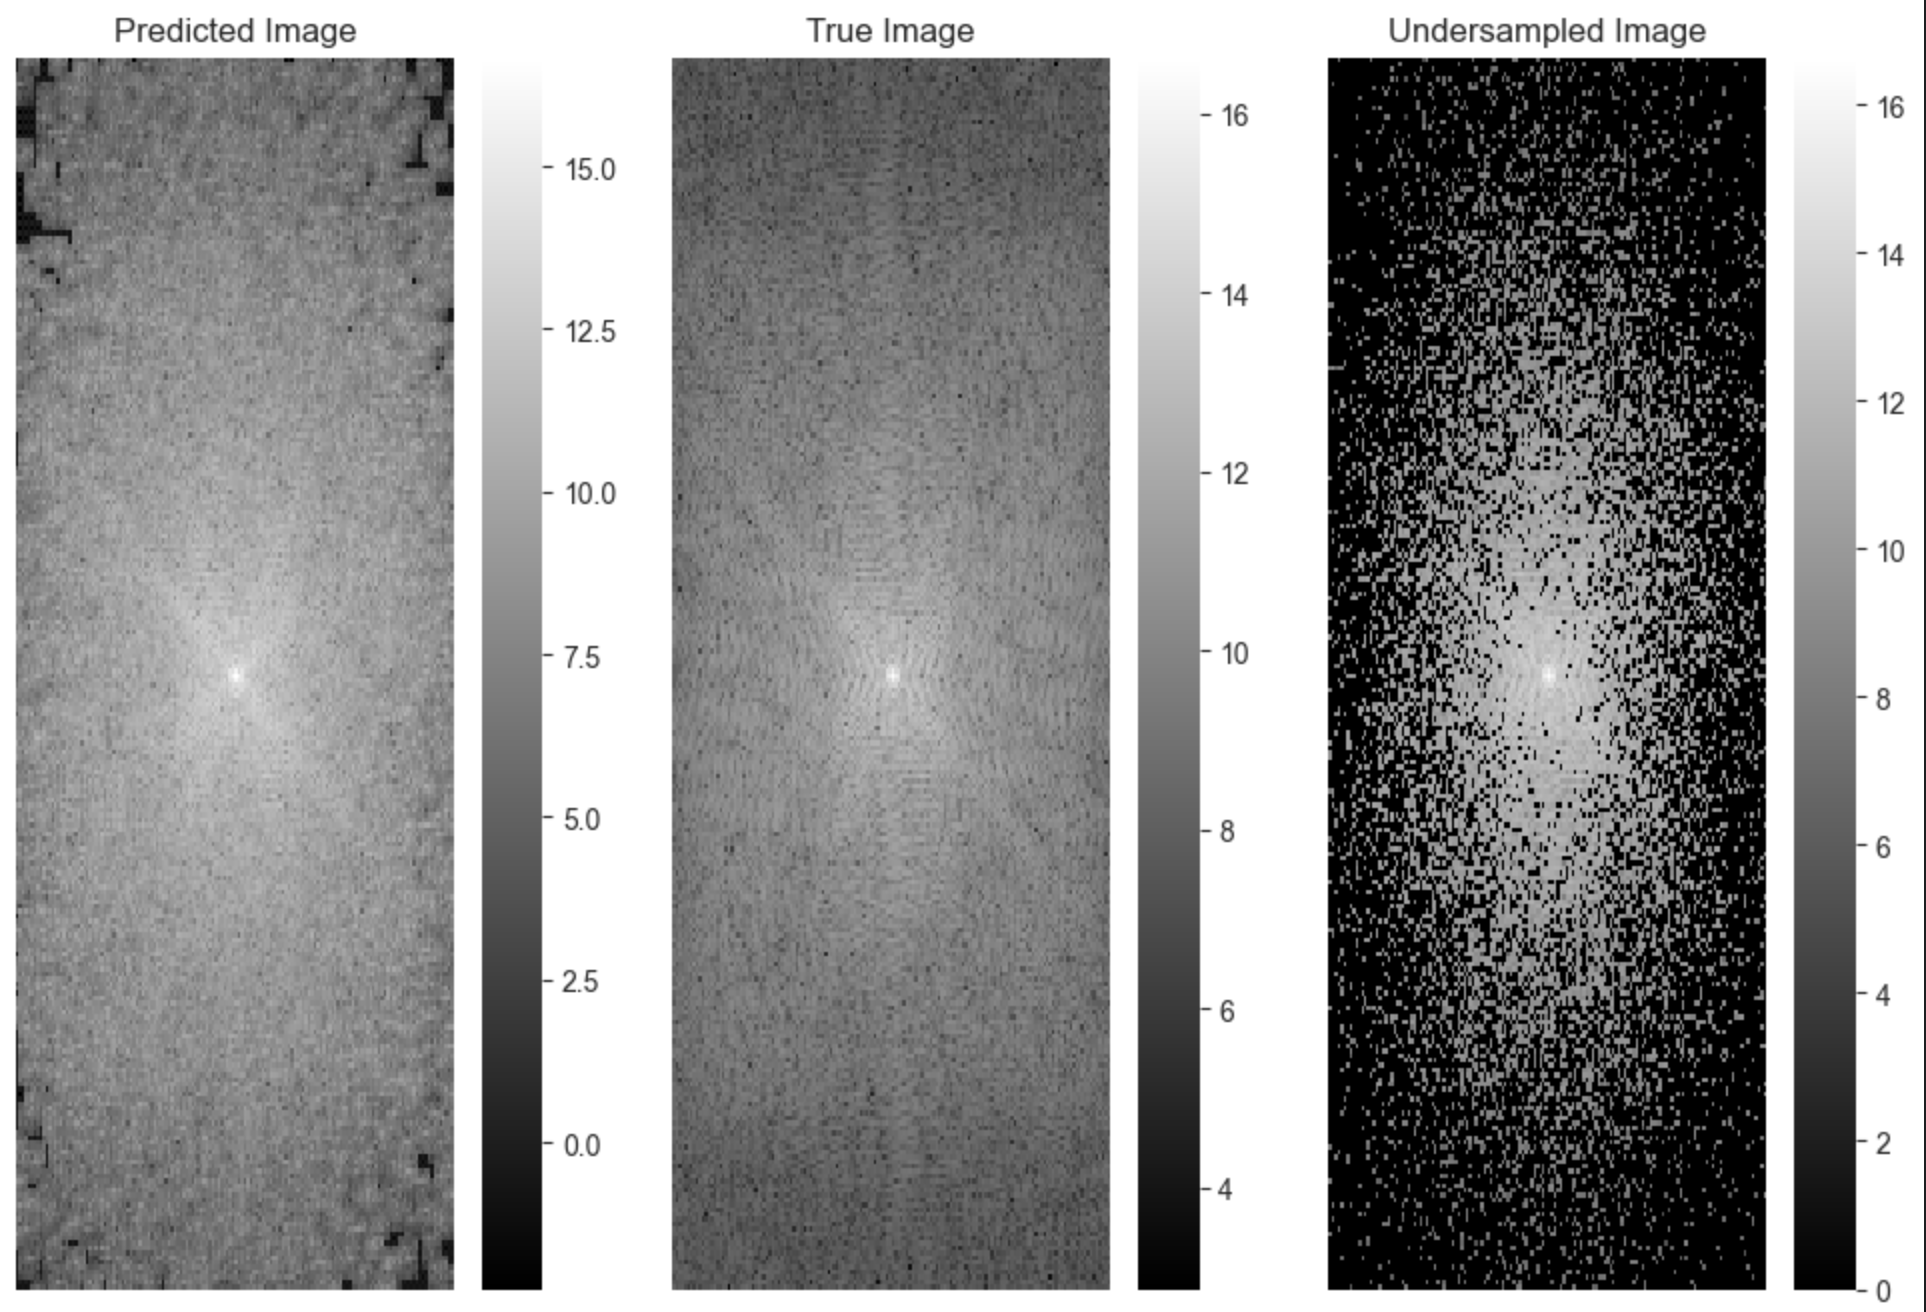
\includegraphics[width=0.75\linewidth]{Kspace-2.png}
            \caption{k-space reconstruction using a CNN for heavily undersampled k-space.}
            \label{img:kspace-2}
        \end{figure}

        It can be shown in figures \ref{img:image-1} and \ref{img:image-2} that this approach is not perfect, but with a deeper model and more training time as well as a larger sample dataset the network shows promise. This is highlighted in figure \ref{img:CNN_1}, where a higher computation time with a larger model was used for the same data as in image \ref{img:image-1}. The key purpose here is to show that the neural networks can successfully reconstruct k-space image trends accurately.

        \begin{figure}[h]
            \centering
            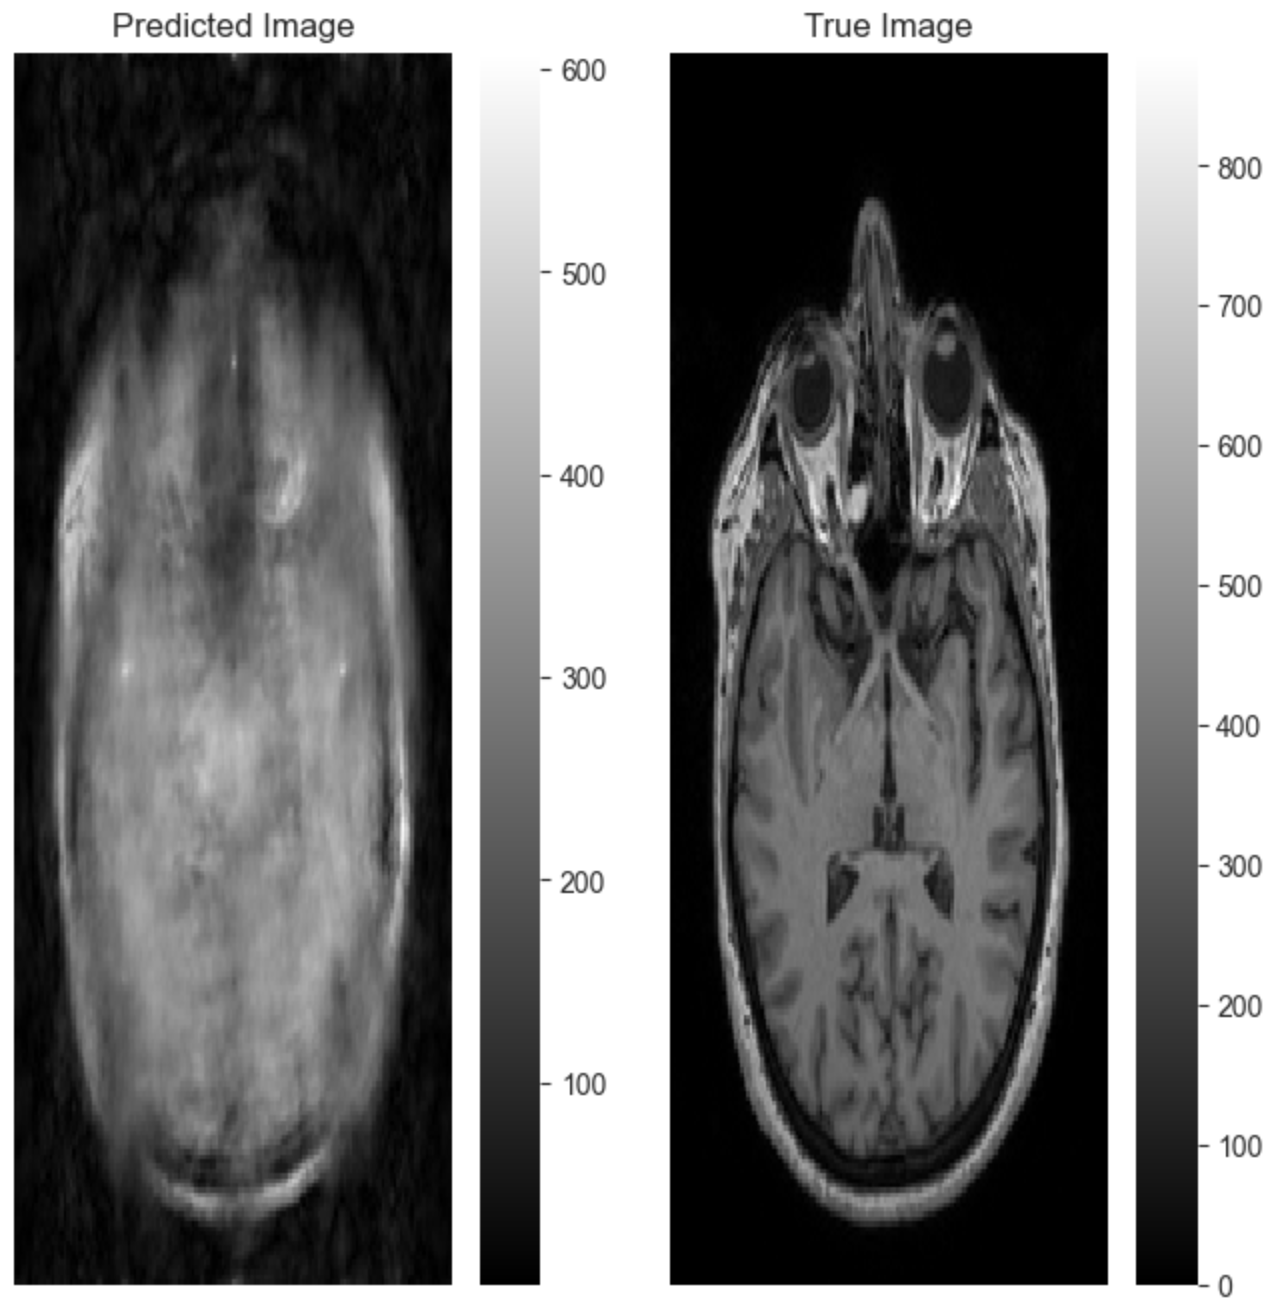
\includegraphics[width=0.5\linewidth]{Image_2.png}
            \caption{k-space reconstruction using a CNN for highly undersampled k-space.}
            \label{img:image-1}
        \end{figure}

        \begin{figure}[h]
            \centering
            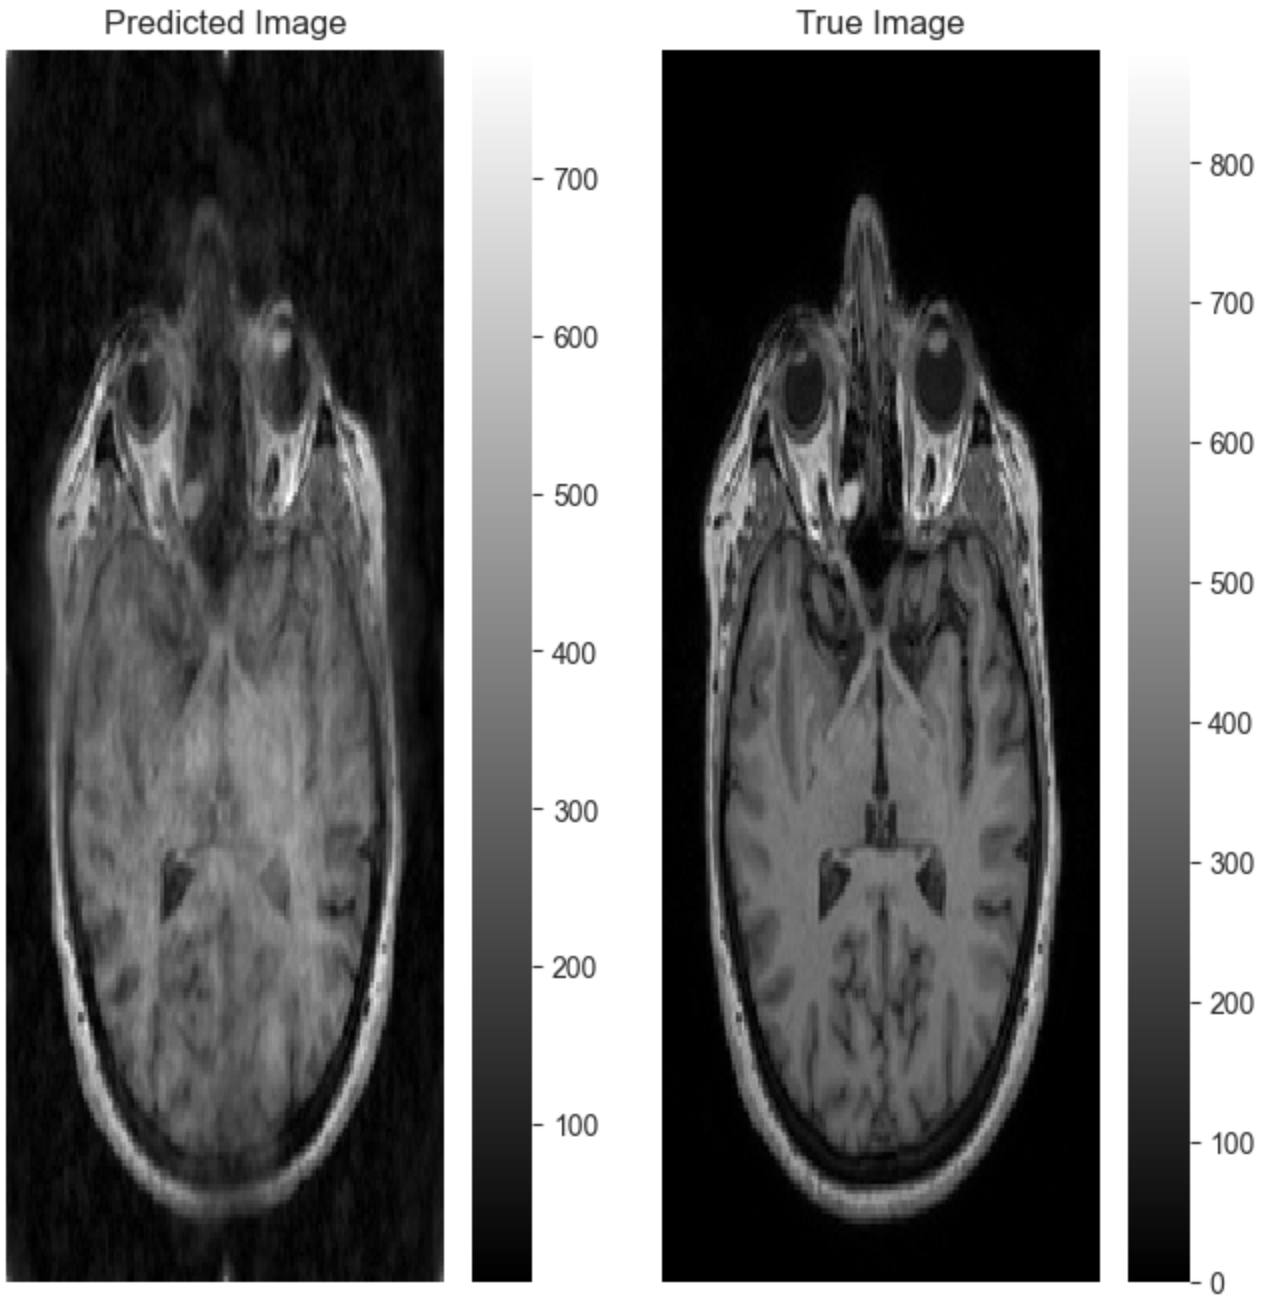
\includegraphics[width=0.39\linewidth]{CNN_1.png}
            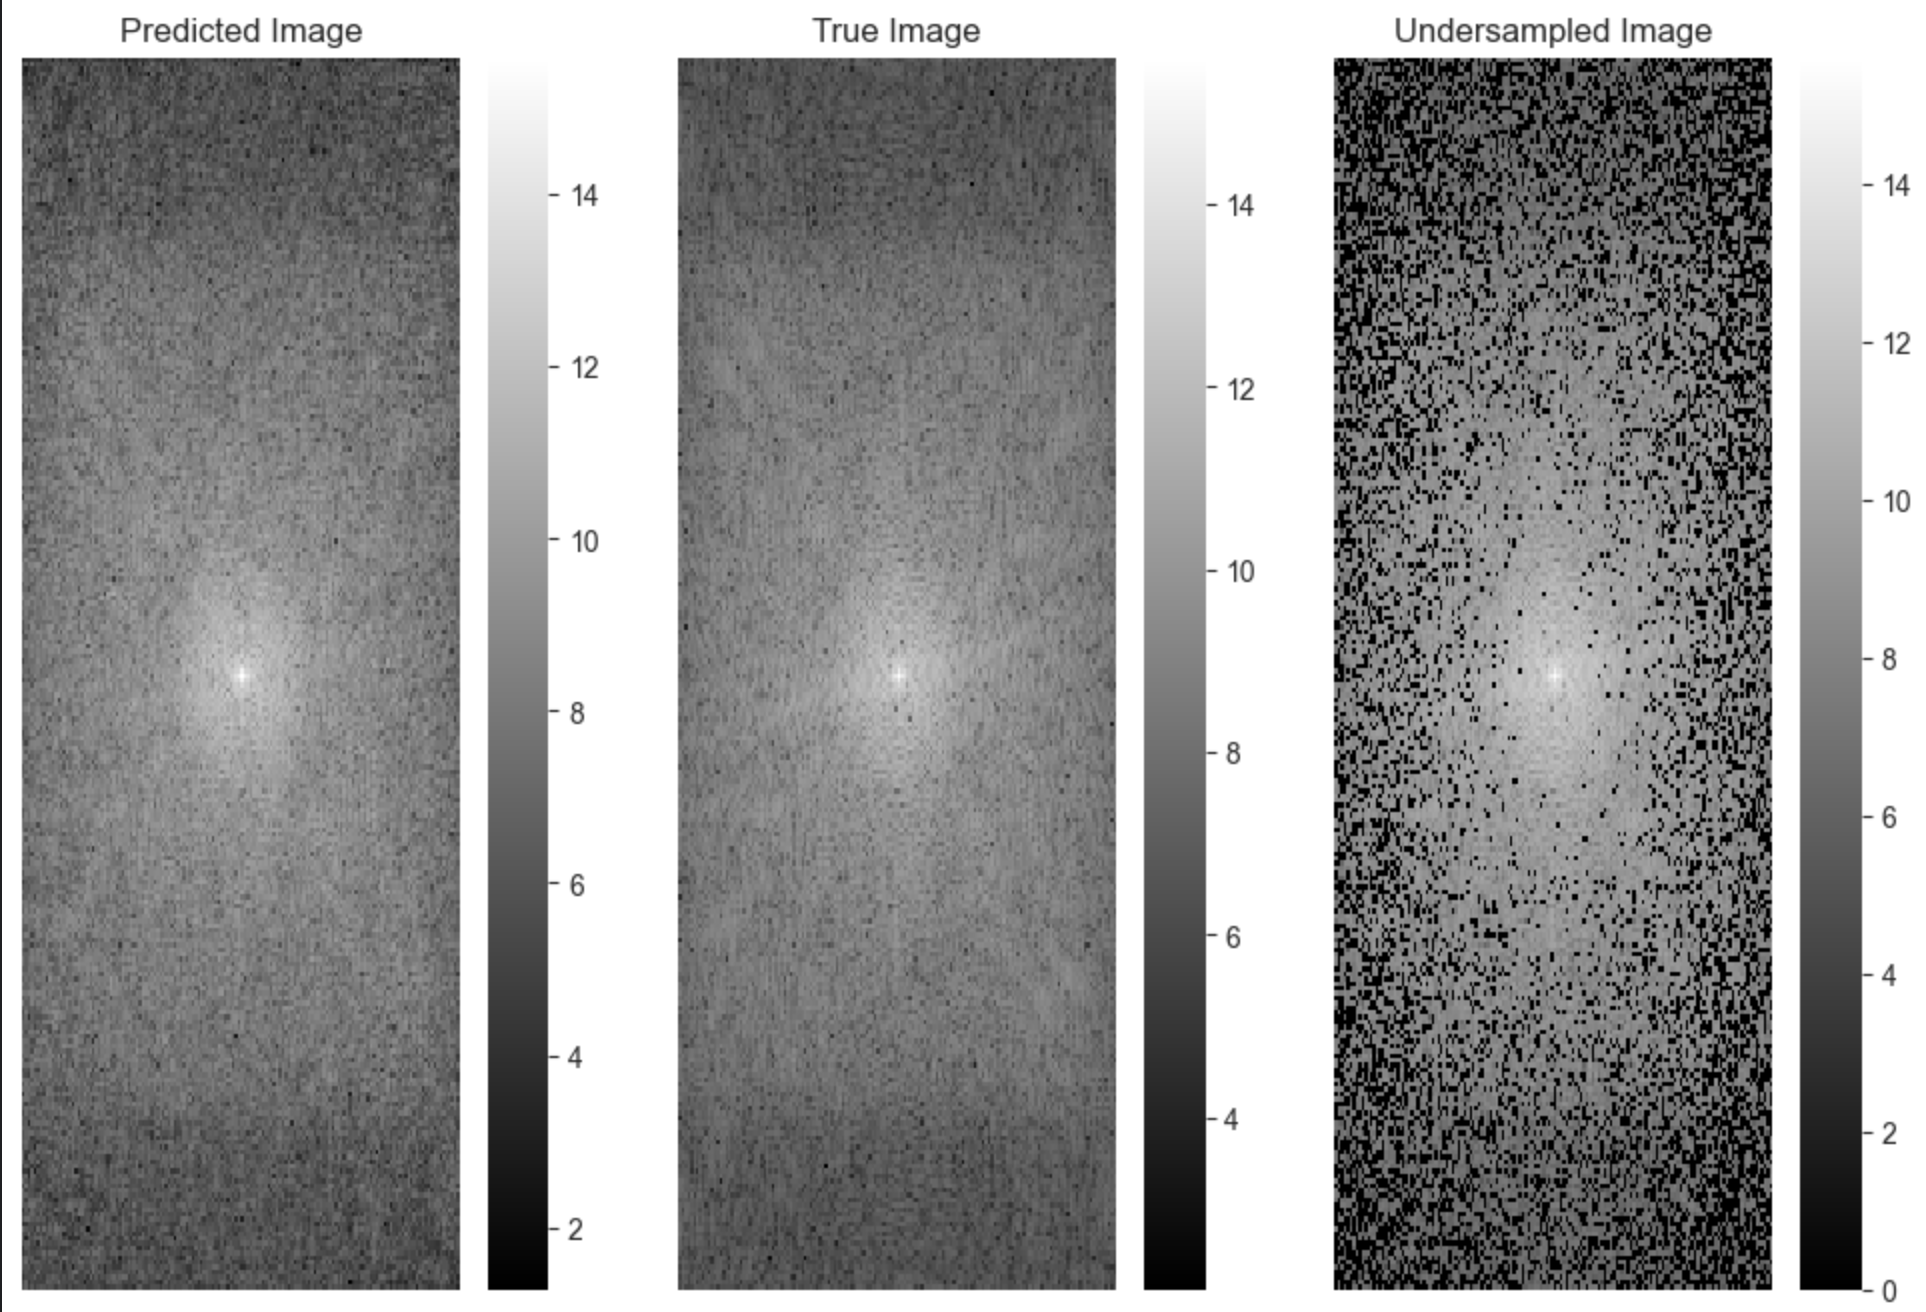
\includegraphics[width = 0.58\linewidth]{CNN_1_kspace.png}
            \caption{Image data of another sample with higher computation time and a larger CNN.}
            \label{img:CNN_1}
        \end{figure}

        \begin{figure}[h]
            \centering
            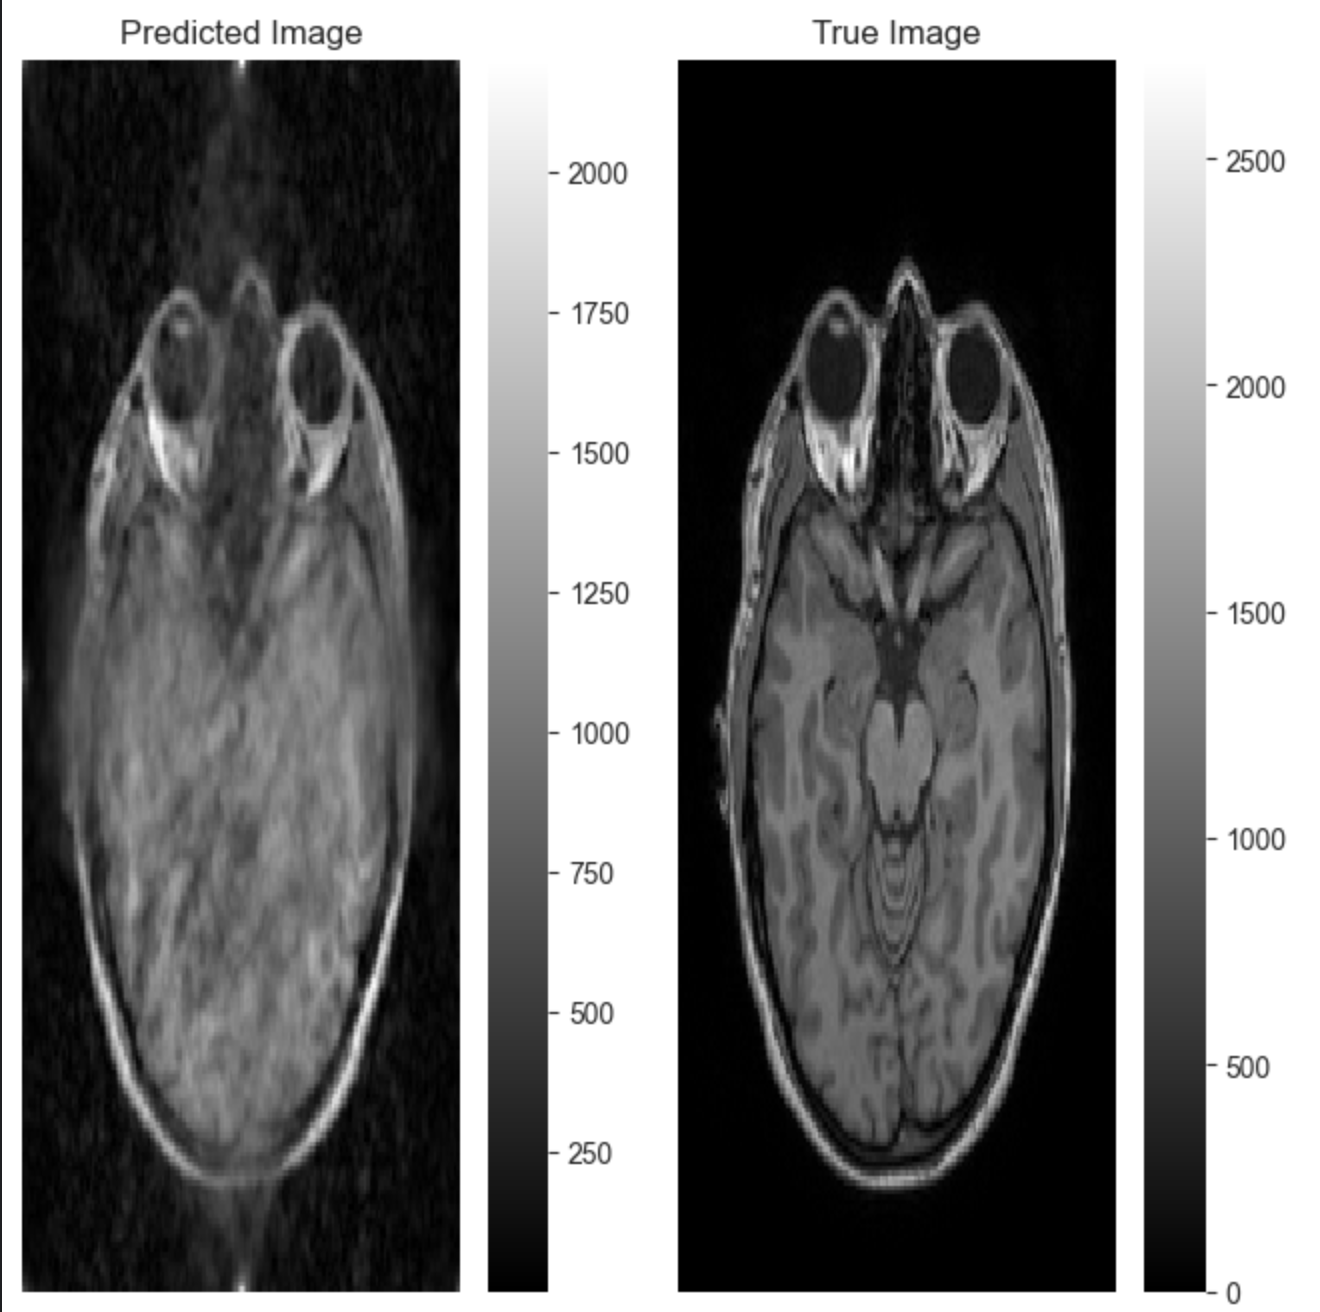
\includegraphics[width=0.5\linewidth]{Image-1.png}
            \caption{k-space reconstruction using a CNN for medium intensity undersampled k-space.}
            \label{img:image-2}
        \end{figure}

        The power of this image processing technique works for any scan, as long as the model is properly trained and not overfitting. Research has shown that CNNs are capable of image enhancement and reconstruction for $T_1$ and $T_2$ weighted images for a variety of sizes and orientations \cite{Wang_Su_Ying_Peng_Zhu_Liang_Feng_Liang_2016}. These models will only grow in predictive power as more image data becomes available for study. A current issue in this area of research is that MRI scan datasets including k-space data is scarce, and models are typically trained on smaller datasets up to $500$ images \cite{Wang_Su_Ying_Peng_Zhu_Liang_Feng_Liang_2016}. An increase in abundance of MRI k-space sampling data will provide the model more information to learn from, which may help it to more accurately produce correct and high quality images.

        It should be discussed that the approach presented by the small model in this paper is nonstandard. Typically, k-space data is transmitted to image data first, before the CNN is trained on the data \cite{Wang_Su_Ying_Peng_Zhu_Liang_Feng_Liang_2016}. Both approaches have their benefits and drawbacks, but this approach is focused on reconstructing the frequency data. Prioritizing frequency data gives the model more information about phase and signal strength, while prioritizing image data prioritizes features of the image. These are not unrelated since they are linked via the \hl{Fourier} transform depicted in equation \eqref{fft}, but the model will learn different skills while presented with different data. A future extension of this project would be to perform the FFT (\hl{Fast-Fourier Transform}) first, then train the CNN on the true image data, and try to reconstruct its features from there. Another future extension of the project would be to analyze how the image reconstruction improves if given not only the \hl{$T_1$-weighted} images, but also the \hl{$T_2$-weighted} images and the $PD$ weighted images. Providing a larger sample size will increase the likelihood that the model can better reconstruct frequency information. This comes at a heavy cost of computation time, computational resources, and memory. These CNN's on average took between 30 minutes to an hour to run on \hl{an Apple Macbook Air M2 with 16Gb of unified memory}. Increasing the information in the dataset would stretch these calculation times much further. This can be circumvented by utilizing GPU programming, but that is a topic outside the scope of this report and can be inveestigated in a future study.

        \hl{Additionally, these models have clinical limitations that need to be highlighted and discussed, such as their immediate application in clinical setting. Currently, neural networks and other machine learning algorithms are not used in the clinical setting. This is due to several factors which include the small datasets the models are trained on as mentioned previously, as well as the repurcussions of an overfit model. Highly complex models are extremely sensitive to overfitting, and if doctors rely on the image processing done by these models, there is a chance of misdiagnosis, which could have serious effects on patient care and health. Larger datasets and further careful training is required before such models can be implemented in a clinical setting. Having a larger dataset allows for a bigger sample size of images for models to learn from, which not only can reduce underfitting, but can help provide more reliable results. When training a CNN, it is important to consider generalization and overfitting in the model analysis. Without careful consideration of model complexity, image artifacts, blurring, and smoothing effects are likely to emerge.}
    
    \section*{Conclusion}
        In conclusion it has been shown that neural networks can serve as a powerful tool for reducing the amount of frequency domain acquisition needed from MRI scans to produce meaningful images of a sample. By training a neural network to analyze the frequency domain data and predict the missing acquisition data for a soft tissue sample it is possible to reconstruct the image without aliasing and significant loss of contrast. 

        As the area of research grows, more complex and larger datasets will become available, allowing for further advanced training of the Concurrent Neural Networks. The application of CNNs in the medical field for MRI imaging has the power to reduce data acquisition times and allow for more patients to be treated via MRI. This can help in the identification of cancerous cells and other tumours in the samples being studied and allow MRI to become a more accessible imaging technique to those in need.
    % \appendix


    % \widetext
    % \section*{Python Code}

    % \begin{python}

    % \end{python}
    % \endwidetext
    \bibliographystyle{IEEEtran}
    \bibliography{citations}

\end{document}
